\documentclass[xcolor={dvipsnames,usenames}]{beamer}
%\documentclass[xcolor={dvipsnames,usenames},handout]{beamer} % use this to compile w/o pauses
\mode<presentation>
{
\usetheme{Madrid}
\usecolortheme{default}
\setbeamertemplate{itemize items}[default]
\setbeamertemplate{enumerate items}[default]
\setbeamercovered{transparent}
\usefonttheme[onlymath]{serif}
}

\usepackage{microtype}
\usepackage[normalem]{ulem}
%\usepackage{hyperref}
%\hypersetup{colorlinks=true, urlcolor=Blue, citecolor=Green, linkcolor=BrickRed, breaklinks, unicode}
\usepackage{textpos}

\usepackage[nocompress]{cite}
\usepackage{amsmath,mathtools}
\usepackage{euscript}
\usepackage{latexsym}
\usepackage{amssymb,stmaryrd}
\usepackage{enumerate}
\usepackage{algorithm,algorithmicx}
\usepackage[noend]{algpseudocode}
\renewcommand{\algorithmicrequire}{\textbf{Requirement:}}

\usepackage{graphicx}
\usepackage{epstopdf}
\usepackage{subcaption}
\graphicspath{{./fig/}}


\title{Efficient Algorithms for Geometric Partial Matching}
\author[Allen Xiao]
{
	Pankaj~K.~Agarwal \and
	Hsien-Chih~Chang \and
	Allen~Xiao
}
\institute[SoCG 2019]
{
	Department of Computer Science, Duke University
}
\date{June 2019}

% tweak wd=X\paperwidth to modify the footer dimensions in the madrid theme
\makeatletter
\setbeamertemplate{footline}{
  \leavevmode%
  \hbox{%
  \begin{beamercolorbox}[wd=.25\paperwidth,ht=2.25ex,dp=1ex,center]{author in head/foot}%
    \usebeamerfont{author in head/foot}\insertshortauthor\expandafter\ifblank\expandafter{\beamer@shortinstitute}{}{~~(\insertshortinstitute)}
  \end{beamercolorbox}%
  \begin{beamercolorbox}[wd=.55\paperwidth,ht=2.25ex,dp=1ex,center]{title in head/foot}%
    \usebeamerfont{title in head/foot}\insertshorttitle
  \end{beamercolorbox}%
  \begin{beamercolorbox}[wd=.2\paperwidth,ht=2.25ex,dp=1ex,right]{date in head/foot}%
    \usebeamerfont{date in head/foot}\insertshortdate{}\hspace*{2em}
    \insertframenumber/\inserttotalframenumber \hspace*{2ex}
  \end{beamercolorbox}}%
  \vskip0pt%
}
\makeatother

% student presentation bg image
\addtobeamertemplate{frametitle}{}{%
\begin{textblock*}{100mm}(.95\textwidth,-0.9cm)

\includegraphics[height=0.8cm,width=0.8cm]{StudentPresentation}
\end{textblock*}}


% make tables less packed
\renewcommand{\arraystretch}{1.5}
% get rid of caption labels
%\setbeamertemplate{caption}{\raggedright\insertcaption\par}
%\captionsetup[subfigure]{labelformat=empty}
% set beamer highlight color (alert)
\setbeamercolor{alerted text}{fg=BrickRed}

\newcommand{\mycite}[1]{{\color{LimeGreen}\lbrack #1\rbrack}}
\newcommand{\etal}{\textit{et~al.}}
\newcommand{\softO}{\widetilde{O}}
\newcommand{\reals}{\mathbb{R}}
\newcommand{\ints}{\mathbb{N}}
\newcommand\nats{\mathbb{N}}
\newcommand{\eps}{\varepsilon}
\DeclareMathOperator{\polylog}{polylog}
\DeclareMathOperator{\poly}{poly}
\newcommand{\flr}[1]{{\lfloor #1\rfloor}}
\DeclareMathOperator*{\argmax}{arg\,max}
\DeclareMathOperator*{\argmin}{arg\,min}
\DeclareMathOperator{\Vor}{Vor}
\DeclareMathOperator{\VorRegion}{VorRegion}

\def\abs#1{\mathopen| #1 \mathclose|}		% use instead of $|x|$
\def\norm#1{\mathopen\| #1 \mathclose\|}	% use instead of $\|x\|$

\def\arcto{\mathord\shortrightarrow}
\def\arc#1#2{#1\arcto#2}

\DeclareMathOperator{\cost}{cost}
\newcommand{\tsupply}{\lambda}
\newcommand{\fsupply}{\phi}

\newcommand{\A}{{\color{red}A}}
\newcommand{\B}{{\color{blue}B}}
\newcommand{\M}{\EuScript{M}}
\newcommand{\tildeM}{\widetilde{\EuScript{M}}}
\newcommand{\X}{\EuScript{X}}

\def\EMPH#1{\textcolor{BrickRed}{{\emph{#1}}}}



\begin{document}


\begin{frame}
\maketitle
\end{frame}

%1. Gentle example
%2. Formal description/dual description
%3. Some previous works comments, our alg time bounds
%4. Ramshaw-Tarjan: Hung at k steps works (also, a cost-scaling algorithm)
%5. Cost-scales/theta-opt outline
%6. Reduction main ideas (integrality issue), sufficient initial condition, theta_under
%7. Within a scale: O(k) excess refined into a circulation (mention blocking flow bound)
%8. High-level goals: after O(npolylogn) preprocessing, execute refinement in O(kpolylogn) time per blocking flow
%9. Refinement descr: Hung search + dfs
%10. Brief review of Hung search (maybe cut), with potential, and BCP
%11. Can't initialize the BCPs for every Hung search, rewind instead (example)
%12. Hungarian search looks at useless things (example)
%13. Dead/alive classification, alive paths
%14. Relaxation with alive paths
%15. Maybe? Details about potential bookkeeping


% INTRO

% 01: gentle example, emphasize cost fn, and q>1
\begin{frame}{Geometric (bipartite) matching}
% two point sets in 2d, show cost fn (distance exponentitated to constant)
\begin{figure}
\begin{center}
\includegraphics<1>[width=0.8\textwidth,page=1]{example}%
\includegraphics<2>[width=0.8\textwidth,page=2]{example}%
\includegraphics<3->[width=0.8\textwidth,page=3]{example}%
\end{center}
\end{figure}
\end{frame}

\begin{frame}{Geometric (bipartite) partial matching}
% only k pairs
\begin{figure}
\begin{center}
\includegraphics<1->[width=0.8\textwidth,page=4]{example}%
\end{center}
\end{figure}
\end{frame}

% 02: comments on prior work
\begin{frame}{Prior work}
\begin{center}
\resizebox{\textwidth}{!}{%
\begin{tabular}{l | c | c | c}
	& \textbf{approx.} & \textbf{time} & \textbf{valid $q$} \\
	\hline
	Hungarian algorithm (Kuhn) & exact & $O(k m + k^2 \log n)$ & $q\geq 1$ \\
		& & $O(kn\polylog n)$ & \\
	Ramshaw, Tarjan 2012 & exact\footnotemark & $O(m\sqrt{k}\log(kC))$ & $q\geq 1$ \\
		& $(1+\eps)$ & $O(n\sqrt{k}\polylog n \log(1/\eps))$ & \\
	\hline
	Sharathkumar, Agarwal 2012 & $(1+\eps)$ & $O(n\poly(\log n, 1/\eps)$ & $q=1$ \\
	\hline
	new (Hungarian) & $1$ & $O((n + k^2)\polylog n)$ & $q \geq 1$ \\
	new (cost-scaling) & $(1+\eps)$ & $O((n + k\sqrt{k})\polylog n \log(1/\eps))$ & $q \geq 1$ \\
\end{tabular}
}
\end{center}
\footnotetext[1]{Assuming integer costs $\leq C$.}
\end{frame}

% 03: as flow
\begin{frame}{Unit-capacity min-cost flow formulation}
\begin{figure}
\begin{center}
\includegraphics<1>[width=\textwidth,page=1]{pm-to-mcf}%
\includegraphics<2>[width=\textwidth,page=2]{pm-to-mcf}%
\includegraphics<3>[width=\textwidth,page=3]{pm-to-mcf}%
\includegraphics<4>[width=\textwidth,page=4]{pm-to-mcf}%
\includegraphics<5>[width=\textwidth,page=5]{pm-to-mcf}%
\includegraphics<6>[width=\textwidth,page=6]{pm-to-mcf}%
\includegraphics<7>[width=\textwidth,page=7]{pm-to-mcf}%
\includegraphics<8->[width=\textwidth,page=8]{pm-to-mcf}%
\end{center}
\end{figure}
\end{frame}

% LP comments
\begin{frame}{Flow terminology}
%TODO replace figure with mcf rotating definitions
\begin{figure}
\begin{center}
\includegraphics[width=0.4\textwidth,page=8]{pm-to-mcf}%
\end{center}
\end{figure}
\vspace{5pt}
\begin{itemize}
%\item \alert{Pseudoflow} may have imbalance, \alert{circulations} are balanced
\item $\alert{c_\pi(\arc vw)} \coloneqq c(\arc vw) - \pi(v) + \pi(w)$
\item \alert{$\theta$-optimality}: $c_\pi(\arc vw) \geq -\theta$ on all residual arcs
\item \alert{admissible} residual arcs: $c_\pi(\arc vw) \leq 0$ 
\end{itemize}
\end{frame}

% LP comments
%\begin{frame}{Dual formulation and terminology}
%TODO figure of LPs
%\begin{equation*}
%\begin{array}{rll}
%\displaystyle\min_{f} & \displaystyle\sum_{\arc vw} c(\arc vw) \cdot f(\arc vw) & \\
%\text{s.t.} & \displaystyle\sum_{u:(\arc uv) \in E} f(\arc uv) - \sum_{w:(\arc vw) \in E} f(\arc vw) = 0 & \forall v \in A\cup B \\
%	& \displaystyle\sum_{a \in A} f(\arc sa) = k & \\
%	& \displaystyle\sum_{b \in B} f(\arc bt) = k & \\
%	& f(\arc vw) \in \{0, 1\} & \forall (\arc vw) \in E \\
%\end{array}
%\end{equation*}
%\end{frame}

% 05 cost scaling
\begin{frame}{Cost-scaling (Ramshaw-Tarjan)}
\begin{itemize}
\item \alert{$\theta$-optimality}: $c_\pi(\arc vw) \geq -\theta$ on all residual arcs
\item \alert{admissible} residual arcs: $c_\pi(\arc vw) \leq 0$ 
\vspace{15pt}
\item $\theta$-optimal circulation is $+n\theta$ approx.
\vspace{15pt}
\item Find $\theta$-optimal circulations for geometrically decreasing values of $\theta$:
	\begin{enumerate}
	\item Reduce $\theta \gets \theta/2$, while creating $O(k)$ excess.
	\item \alert{Refine} this pseudoflow into a circulation, while preserving $\theta$-optimality
	\end{enumerate}
\end{itemize}
\end{frame}

% 06 reduction
\begin{frame}{Cost-scaling for geometric partial matching}
%TODO add a pic showing intra-cluster k-matching
\begin{figure}
\begin{center}
\includegraphics<1>[width=0.7\textwidth,page=1]{single-linkage_clustering}%
\includegraphics<2>[width=0.7\textwidth,page=2]{single-linkage_clustering}%
\includegraphics<3->[width=0.7\textwidth,page=3]{single-linkage_clustering}%
\end{center}
\end{figure}
\begin{itemize}
\item<4-> There exists a $k$-matching whose longest edge is $(n^q\cdot\alpha)$, and a $(\eps\alpha/6k)$-optimal circulation is $(1+\eps)$-approx.
\item<5-> $(1+\eps)$-approx. geometric partial matching reduces into executing $O(\log(n^q/\eps))$ cost scales.
\end{itemize}
\end{frame}

% 07 within a scale (blocking flow bound)
\begin{frame}{Refinement by blocking flows (Ramshaw-Tarjan)}
\begin{itemize}
\item Inside Refine:
	\begin{enumerate}
	\item Hungarian search: raise potentials until an excess-deficit admissible path exists.
	\item Augment by an admissible \alert{blocking flow}.
	\end{enumerate}
\begin{figure}
\begin{center}
\includegraphics<1>[width=0.7\textwidth,page=1]{blocking_flow}%
\includegraphics<2>[width=0.7\textwidth,page=2]{blocking_flow}%
\includegraphics<3>[width=0.7\textwidth,page=3]{blocking_flow}%
\includegraphics<4->[width=0.7\textwidth,page=4]{blocking_flow}%
\end{center}
\end{figure}
\item<5-> $O(\sqrt{k})$ blocking flows before $f$ becomes a circulation.
\end{itemize}
\end{frame}

% 08 high-level goals for runtime
% 09 refinement description (h.s. + dfs)
\begin{frame}{High-level goal per scale}
\begin{itemize}
\item Inside Refine:
	\begin{enumerate}
	\item Hungarian search: raise potentials until an excess-deficit admissible path exists.
	\item Augment by an admissible \alert{blocking flow}.
	\end{enumerate}
\vspace{15pt}
\item After $O(n\polylog n)$-time preprocessing, perform Hungarian search and find each blocking flow in $O(k\polylog n)$ time.
\end{itemize}
\end{frame}

\begin{frame}{Hungarian search with BCP (Agarwal-Efrat-Sharir)}
\begin{figure}
\begin{center}
\includegraphics<1>[width=0.9\textwidth,page=1]{hung_search}%
\includegraphics<2>[width=0.9\textwidth,page=2]{hung_search}%
\includegraphics<3>[width=0.9\textwidth,page=3]{hung_search}%
\includegraphics<4>[width=0.9\textwidth,page=4]{hung_search}%
\includegraphics<5>[width=0.9\textwidth,page=5]{hung_search}%
\includegraphics<6>[width=0.9\textwidth,page=6]{hung_search}%
\includegraphics<7>[width=0.9\textwidth,page=7]{hung_search}%
\includegraphics<8>[width=0.9\textwidth,page=8]{hung_search}%
\includegraphics<9->[width=0.9\textwidth,page=9]{hung_search}%
\end{center}
\end{figure}
\begin{itemize}
\item<4-> Dynamic 2D BCP with $O(\polylog n)$ update time, $O(\log^2 n)$ query time (Kaplan~{\etal} SODA'17)
\end{itemize}
\end{frame}

% 12 hung search looks at useless
\begin{frame}{Problem: Hungarian search looks at too many nodes}
\begin{figure}
\begin{center}
\includegraphics<1>[width=0.9\textwidth,page=1]{why_dead}%
\includegraphics<2>[width=0.9\textwidth,page=2]{why_dead}%
\includegraphics<3>[width=0.9\textwidth,page=3]{why_dead}%
\includegraphics<4->[width=0.9\textwidth,page=4]{why_dead}%
\end{center}
\end{figure}
\end{frame}

% 13 dead/alive
\begin{frame}{Dead/alive nodes}
\begin{itemize}
\item \alert{Alive nodes}: nonzero excess/deficit, or adjoining flow support arcs.
\item \alert{Dead nodes}: ones which aren't alive.
\begin{figure}
\begin{center}
\includegraphics<1>[width=0.8\textwidth,page=5]{why_dead}%
\includegraphics<2>[width=0.8\textwidth,page=6]{why_dead}%
\includegraphics<3,4>[width=0.8\textwidth,page=7]{why_dead}%
\includegraphics<5>[width=0.8\textwidth,page=8]{why_dead}%
\includegraphics<6->[width=0.8\textwidth,page=9]{why_dead}%
\end{center}
\end{figure}
\item<4-> \alert{Alive path}: residual path between two alive nodes with no other alive nodes in between.
\item<7-> Don't need to track potential of dead nodes.
\end{itemize}
\end{frame}

% 14 relaxing alive paths
\begin{frame}{Relaxing alive paths}
\begin{itemize}
\item Alive paths have length 1, 2, or 3.
\begin{figure}
\begin{center}
\includegraphics<1>[width=0.7\textwidth,page=1]{alive_paths}%
\includegraphics<2>[width=0.7\textwidth,page=2]{alive_paths}%
\includegraphics<3>[width=0.7\textwidth,page=3]{alive_paths}%
\includegraphics<4>[width=0.7\textwidth,page=4]{alive_paths}%
\includegraphics<5->[width=0.7\textwidth,page=5]{alive_paths}%
\end{center}
\end{figure}
\item<5-> Telescoping: $c_\pi(s \arcto a \arcto b) = c(\arc ab) - \pi(s) + \pi(b)$ (use BCP)
\item<6-> Only $O(k)$ relaxations per Hungarian search.
\item<7-> Also: find a blocking flow in $O(k)$ relaxations (DFS).
\end{itemize}
\end{frame}

% 11 problem with bcp init
\begin{frame}{Problem: BCP initialization}
\begin{itemize}
\item Dynamic 2D BCP with $O(\polylog n)$ update time, $O(\log^2 n)$ query time (Kaplan~{\etal} SODA'17)
\begin{figure}
\begin{center}
\includegraphics[width=0.8\textwidth,page=6]{why_dead}%
\end{center}
\end{figure}
\item Some BCP may begin a Hungarian search with $\Theta(n)$ vertices.
\item Can't afford to construct from scratch for every Hungarian search.
\end{itemize}
\end{frame}

\begin{frame}{Initial BCP by rewinding}
\begin{figure}
\begin{center}
\includegraphics<1>[width=0.8\textwidth,page=1]{bcp_init}%
\includegraphics<2>[width=0.8\textwidth,page=2]{bcp_init}%
\includegraphics<3>[width=0.8\textwidth,page=3]{bcp_init}%
\includegraphics<4>[width=0.8\textwidth,page=4]{bcp_init}%
\includegraphics<5>[width=0.8\textwidth,page=5]{bcp_init}%
\includegraphics<6>[width=0.8\textwidth,page=6]{bcp_init}%
\includegraphics<7->[width=0.8\textwidth,page=7]{bcp_init}%
\end{center}
\end{figure}
\begin{itemize}
\item<7-> $X_t$ and $X_{t+1}$ differ by the newly-matched $A$ nodes.
\item<8-> Generate $X_{t+1}$ by \alert{rewinding} the BCP updates done on $X_t$, then deleting the newly-matched nodes. \\
	Same number of BCP updates as the Hungarian search.
\item<9-> Persistence?
\vspace{10pt}
\item<10-> Construct once ($O(n\polylog n)$), then $O(k\polylog n)$ time to rewind and generate the next BCP.
\end{itemize}
\end{frame}

% 15 potential stuff?
%\begin{frame}
%\end{frame}

% end slide
\begin{frame}{The End}
\begin{center}
	Thank you.
\end{center}
\end{frame}

%\begin{frame}[allowframebreaks]{Citations}
%\tiny
%\bibliography{ref}
%\bibliographystyle{alpha}
%\end{frame}

\end{document}
